\subsubsection{Streuparameter}\label{subsubsec:streuparameter}

Die Streuparameter (S-Parameter) werden in der Hochfreqeunztechnik verwendet, um das Verhalten von n-Toren zu beschreiben. Bei einem 2-Tor sind vier Streuparameter von nöten um das Verhalten zu beschreiben. Sie beschreiben die Transmission von Tor 1 zu Tor 2, sowie von Tor 2 zu Tor 1. Des weiteren zeigen sie die Reflexion an den Toren auf. Abbildung \ref{fig:2-Tor} \nameref{fig:2-Tor} zeigt die Streuparameter an einem 2-Tor. 
\begin{figure}[H]
	\centering
	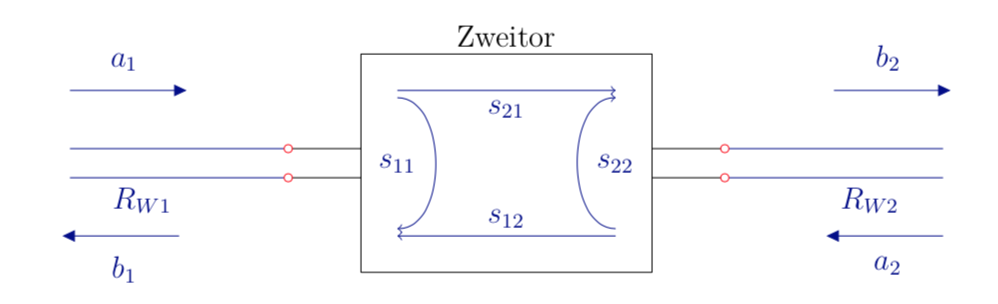
\includegraphics[width=15cm]{s_params_def.png}
	\caption{2-Tor Wellengrössen und Anschlussleitungen \cite{hftech}}
	\label{fig:2-Tor}
\end{figure}
Bei den S-Parameter werden die Eingangs- und Ausgangsgrössen nicht direkt anhand elektrischer Ströme und Spannungen beschrieben. Sie werden mithilfe von Wellengrössen beschrieben, wobei a\textsubscript{i} die einlaufenden Wellen sind und b\textsubscript{i} die Reflektierenden Wellen. Der Index i stellt den Torindex dar. Formel \ref{equ:def_a} und \ref{equ:def_b} zeigen wie die Wellengrössen a\textsubscript{i} sowie b\textsubscript{i} definiert sind. Die Quadrate der Beträge der Wellenstärken a und b entsprechen gerade den Leistungen, die mit diesen Wellen übertragen werden.
\begin{equation}\label{equ:def_a}
	a_{ i } = \sqrt{ P_{ vor } }, a = Wellenstärke der vorlaufenden Welle
\end{equation}
\begin{equation}\label{equ:def_b}
	b_{ i } = \sqrt{ P_{ rück } }, b = Wellenstärke der rücklaufenden Welle
\end{equation}

Aus der Abbildung 2.3 lässt sich folgende Streumatrix darstellen (Formel \ref{equ:scatteringMatrix}):
\begin{equation}\label{equ:scatteringMatrix}
	\left[
		\begin{matrix}b_1 \\ b_2 \end{matrix}
	\right]
 	=
 	\left[
 		\begin{matrix}
			s_{11}&s_{12} \\s_{21}&s_{22}
		\end{matrix}
	\right]
	\cdot 
	\left[
		\begin{matrix}
			a_1\\a_2
		\end{matrix}
	\right]
\end{equation}

Die Elemente der S-Matrix sind:

\begin{equation}\label{equ:def_s11}
	s_{11} = b_1/a_1\textsf{ Eingangsreflexionsfaktor bei angepasstem Ausgang (a\textsubscript{2}=0)}
\end{equation}
\begin{equation}\label{equ:def_s12}
	s_{12} = b_1/a_2\textsf{ Rückwärtstransmissionsfaktor bei angepasstem Eingang (a\textsubscript{1}=0)}
\end{equation}
\begin{equation}\label{equ:def_s21}
	s_{21} = b_2/a_1\textsf{ Vorwärtstransmissionsfaktor bei angepasstem Ausgang (a\textsubscript{2}=0)}
\end{equation}
\begin{equation}\label{equ:def_s22}
	s_{22} = b_2/a_2\textsf{ Ausgangsreflexionsfaktor bei angepasstem Eingang (a\textsubscript{1}=0)}
\end{equation}

An folgender Schaltung \ref{fig:bspscattering} wird Schritt für Schritt erklärt, wie der $s_{21}$-Parameter der Streumatrix berechnet wird. 
\begin{figure}[H]
	\centering
	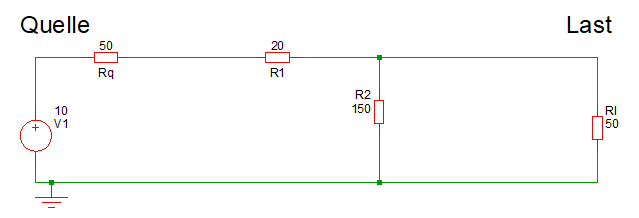
\includegraphics[width=15cm]{bspscattering.png}
	\caption{Beispielschaltung Streuparameter}
	\label{fig:bspscattering}
\end{figure}
Der Streuparameter $s_{21}$ ist, wie in Formel \ref{equ:s21} definiert. Somit muss in einem ersten Schritt die Kettenmatrix der Gesamtschaltung ermittelt werden. Die Kettenmatrix bezieht sich auf die beiden Widerstände $R_1$ und $R_2$. Der Widerstand $R_1$ stellt eine Längsimpedanz dar, welche somit in die passende Matrix eingesetzt wird(Formel \ref{equ:horizImpedance}). $A_1$ (Formel \ref{equ:r1}) stellt die Kettenmatrix der Längsimpedanz $R_1$ dar.
\begin{equation}\label{equ:r1}
	A_1 = \left[\begin{matrix}
			1&R_1\\0&1
			\end{matrix}\right]
\end{equation}

Der Widerstand $R_2$ stellt eine Querimpedanz dar, welche in die Formel \ref{equ:verticImpedance} eingesetzt wird. $A_2$ (Formel \ref{equ:r2}) stellt die Kettenmatrix der Querimpedanz $R_2$ dar.
\begin{equation}\label{equ:r2}
			A_2 = \left[\begin{matrix}
			1&0\\\frac{1}{R_2}&1
			\end{matrix}\right]
\end{equation}

Durch Kaskadieren der beiden Kettenmatrizen wird die Kettenmatrix der Gesamtschaltung gebildet. Kaskadieren bedeutet das Bilden des Matrixproduktes.

\begin{equation}\label{equ:bspSMatrixtot}
A_{tot} = A_1 \cdot A_2 = \left[\begin{matrix}
			1&R_1\\0&1
			\end{matrix}\right] \cdot  \left[\begin{matrix}
			1&0\\\frac{1}{R_2}&1
			\end{matrix}\right]
			= \left[\begin{matrix}
			1&20\\0&1
			\end{matrix}\right] \cdot \left[\begin{matrix}
			1&0\\\frac{1}{150}&1
			\end{matrix}\right] =
			\left[\begin{matrix}
			1.1333&20.000\\0.0067&1.0000
			\end{matrix}\right]
\end{equation}

Der nächste Schritt besteht darin, die Kettenmatrix in Bezug zu den Wellenimpedanzen darzustellen. In diesem Beispiel entspricht die Wellenimpedanz des Innen, sowie Lastwiderstandes mit dem Wert 50 Ohm. Aus der Formel \ref{equ:bspSMatrixtotnorm}  wird diese durch Einsetzen gebildet.

\begin{equation}\label{equ:bspSMatrixtotnorm}
			A'_{tot} = \left[\begin{matrix}
			A_{11}\cdot\sqrt{ \frac{ R_{ l } }{ R_{ q } } }
			&
			\frac{A_{12}}{\sqrt{R_q \cdot R_l}}
			\\
			A_{21} \cdot \sqrt{R_q \cdot R_l}
			&
			A_{22} \cdot \sqrt{\frac{R_q}{R_l}}
			\end{matrix}\right]
			=
			\left[\begin{matrix}
			1.1333\cdot\sqrt{ \frac{ 50}{50} }
			&
			\frac{20.000}{\sqrt{50\cdot 50}}
			\\
			0.0067 \cdot \sqrt{50 \cdot 50}
			&
			1.0000 \cdot \sqrt{\frac{50}{50}}
			\end{matrix}\right]
			=
			\left[\begin{matrix}
			1.1333
			&
			0.4000
			\\
			0.3333
			&
			1.0000
			\end{matrix}\right]
\end{equation}
Aus der Matrix $A'_{tot}$ kann mithilfe der Formel \ref{eqn:s21ausA} der Streuparameter $s_{21}$ direkt ausgerechnet werden.

\begin{equation}\label{eqn:s21ausA}
	s_{21} = \frac{2}{A'_{11}+A'{12}+A'_{21}+A'_{22}}
	=
	\frac{2}{1.1333+0.4000+0.3333+1.0000}
	= 0.6977
\end{equation}
Der Streuparameter $s_{21}$ entspricht dem Transmissionsfaktor der eingehenden Welle. Daraus ergibt sich die Formel \ref{eqn:s32ausLeistung}. Dies dient dient der Überprüfung der vorigen Berechnungen. Die Resultate der beiden Berechnungen stimmen überein.
\begin{equation} \label{eqn:s32ausLeistung}
	s_{21} = \sqrt{ \frac {P_l}{P_{AV}}} = \sqrt{ \frac{0.2434W} {0.5000W}} = 0.6977
\end{equation}
